%%
%% This is file `engagement.tex',
%% The first command in your LaTeX source must be the \documentclass command.
\documentclass[sigconf]{acmart}

%%
%% \BibTeX command to typeset BibTeX logo in the docs
\AtBeginDocument{%
  \providecommand\BibTeX{{%
    \normalfont B\kern-0.5em{\scshape i\kern-0.25em b}\kern-0.8em\TeX}}}

%% Rights management information.  This information is sent to you
%% when you complete the rights form.  These commands have SAMPLE
%% values in them; it is your responsibility as an author to replace
%% the commands and values with those provided to you when you
%% complete the rights form.
\setcopyright{acmcopyright}
\copyrightyear{2021}
\acmYear{2021}
\acmDOI{10.000/0000.0000}

%% These commands are for a PROCEEDINGS abstract or paper.
\acmConference[LAK '21]{LAK '21: Learning 
Analytics \& Knowledge}{April 2021}{UCI,CA}
%\acmBooktitle{Woodstock '18: ACM Symposium on 
%Neural Gaze Detection,
%  June 03--05, 2018, Woodstock, NY}
%\acmPrice{15.00}
%\acmISBN{978-1-4503-XXXX-X/18/06}


%%
%% Submission ID.
%% Use this when submitting an article to a sponsored event. You'll
%% receive a unique submission ID from the organizers
%% of the event, and this ID should be used as the parameter to this command.
%%\acmSubmissionID{123-A56-BU3}

%% end of the preamble, start of the body of the document source.
\begin{document}

%%
%% The "title" command has an optional parameter,
%% allowing the author to define a "short title" to be used in page headers.
\title{Modelling engagement in Technology-mediated 
Peer-Instruction}

\author{Sameer Bhatnagar}
\author{Antoine Lefebvre-Brossard}
\author{Michel C. Desmarais}
\author{Amal Zouaq}
\email{{sameer.bhatnagar,antoine.lefebvre-brossard,michel.desmarais,amal.zouaq}@polymtl.ca}
\affiliation{%
  \institution{Ecole Polytechnique Montreal}
  \country{Canada}
}


\renewcommand{\shortauthors}{Bhatnagar, et al.}

%%
%% The abstract is a short summary of the work to be presented in the
%% article.
\begin{abstract}
\textbf{TO DO}
\end{abstract}

%%
%% The code below is generated by the tool at http://dl.acm.org/ccs.cfm.

\begin{CCSXML}
	<ccs2012>
	<concept>
	<concept_id>10010405.10010489.10010490</concept_id>
	<concept_desc>Applied 
	computing~Computer-assisted 
	instruction</concept_desc>
	<concept_significance>500</concept_significance>
	</concept>
	<concept>
	<concept_id>10010147.10010178.10010179</concept_id>
	<concept_desc>Computing methodologies~Natural 
	language processing</concept_desc>
	<concept_significance>500</concept_significance>
	</concept>
	</ccs2012>
\end{CCSXML}

\ccsdesc[500]{Applied computing~Computer-assisted 
instruction}
\ccsdesc[500]{Computing methodologies~Natural 
language processing}


%%
%% Keywords. The author(s) should pick words that accurately describe
%% the work being presented. Separate the keywords with commas.
\keywords{Peer Instruction, Text Mining}


\maketitle

\section{Introduction}

Technology-mediated peer instruction platforms 
\cite{univeristy_of_british_columbia_ubc/ubcpi_2019}\cite{charles_harnessing_2019}
prompt students to not only answer multiple-choice items, but also provide 
explanations that justify their reasoning. 
Students are then prompted to revise their answer choice by reading some of the 
explanations written by their peers, for another answer choice.
This modality is a specific case of 
\textit{learnersourcing}\cite{weir_learnersourcing_2015}, wherein students 
generate content as part of their own learning process, that is ultimately used 
to help their peers learn as well. 

At this \textit{review step}, students are also presented with peer-written 
explanations for the same answer choice. 
The student now has three options:
\begin{enumerate}
	\item Change their answer choice, by indicating which of their peer's 
	explanations was most convincing
	\item keep their answer choice, but \textit{change explanations} by 
	choosing one that is for the same answer as their own
	\item choose ``I stick to my own'', indicating that their own explanation 
	is best from amongst those that are shown.
\end{enumerate}

In many teaching contexts, teachers do not have the time to review, and provide 
feedback, to every student explanation for every question item. 
The feedback students receive is primarily based on the correctness of their 
first and second answer, not the explanations they write and choose.
Moreover, activities from online learning environments are often used for 
formative assessment, and carry little weight in terms of course credit. 
Framed as a low-stakes test, this can lead to low student 
motivation \cite{wise_low_2005}. 
A version of the expectancy-value model \cite{pintrich_dynamic_1989}, which 
describes factors that influence the effort students will direct towards a 
task, include ``how important they perceive the test to be'', and the 
``affective reaction to how mentally taxing the task appears to be'' 
\cite{wolf_consequence_1995}.

This may explain, in part, the tendency for students to simply ``stick to their 
own'', as shown in figure \ref{fig:sankey}. 
Of the students who choose the correct answer choice on the first step, more 
than half choose their own as ``most convincing'' over the explanations that 
are shown on the \textit{review} step (39\% vs 35\%).
Of those who begin with incorrect answer, and maintain their 
incorrect answer on the review step, we find approximately the same relative 
ratios (9\% vs 8\%).
The last third of these students demonstrate some form of \textit{learning} as 
well, as they transition to the correct answer after reading their peer's 
explanations.

\begin{figure}
	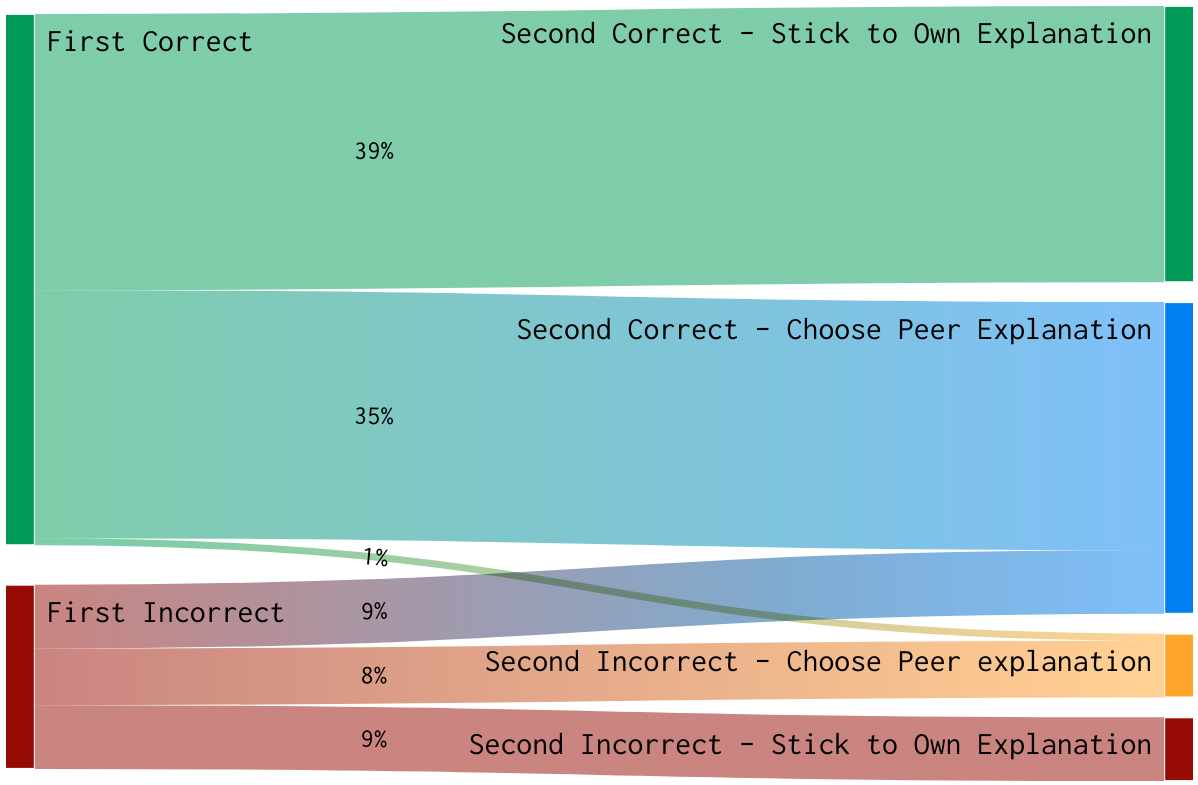
\includegraphics[width=\linewidth]{img/transitions_final}
	\caption{
		Sankey Diagram depicting transitions in peer-instruction 
		platform.
		On the left, responses are separated by whether the student chose the 
		correct answer at the first step, or not.
		For each of these two scenarios, there are three possible transitions 
		towards the right: a) keep the same answer choice, and choose their own 
		explanation, b) keep the same answer choice, and choose a peer's 
		explanation, or c) choose a different answer choice (by choosing a 
		peer's explanation for the other answer choice option presented)
		\textbf{TO DO}: make diagram for different 
		disciplines
	}
	\label{fig:sankey}
\end{figure}

These numbers suggest that when a student chooses a peer's explanation as more 
convincing than their own, for the same answer choice, this ``vote'' that has 
been cast, can be interpreted as a proxy for learner \textit{engagement}.

In this work, we suggest that if we can accurately model when students 
\textit{change} explanations, we may have proxy for student 
\textit{engagement}. 


\section{Related Work}

\subsection{Engagement}


\subsection{Modelling Argument Persuasiveness}




\section{Methodology}



\subsection{Engagement}


\begin{equation}
Engagement_{student} = 
\overline{P(ChosenExplanation \ne 
	OwnExplanation)} 
\label{eq:engagement_choose_peer}
\end{equation}



\subsection{Features}


\subsubsection{Surface Features}

	\begin{enumerate}
	\item Word count of explanation that the student wrote 
	\item Word counts of explanations that were shown on the review step
	\item Number of explanations shown that were much shorter, or much longer 
	than than the student's own explanation 
	\item First answer correct
%	\item time spent writing
	\end{enumerate}


\subsubsection{Convincingness Features}
Two measures of \textit{convincingness} are explored in this work:
\begin{enumerate}
	\item \textbf{Win Rate}: a heuristic measure \cite{potash_ranking_2019}
	\item \textbf{Bradley-Terry}
\end{enumerate}


\begin{acks}
\textbf{TO DO}
\end{acks}

\bibliographystyle{ACM-Reference-Format}
\bibliography{MyLibrary}

\end{document}
\endinput
%% End of file `engagement.tex'.

%%%%%%%%%%%%%%%%%%%%%%%%%%%%%%%%%
% ARCHIVE

%\subsection{Text-to-text similarity}
%Many of the features in our models are based on 
%similarity 
%metrics between 
%student explanations with each other, as well as 
%with other 
%references. 
%
%Consideration must be taken in choosing a metric 
%for measuring 
%similarity 
%between two texts. 
%The use of cosine similarity is standard practice 
%in Latent 
%Semantic 
%Indexing,
%
%\begin{equation}
%sim(T_1,T_2) = \frac{T_1 \cdot T_2}{\| T_1 \| \| 
%	T_2 \|}
%\end{equation}
%
%where $T_1$ and $T_2$ are the \textit{Tf-Idf} 
%vector 
%representations of 
%each text.
%
%However there is extensive work on text-to-text 
%similarity 
%metrics 
%\cite{mihalcea_corpus-based_2006}, 
%which can be divided into two families:
%\begin{enumerate}
%	\item Knowledge Based:
%	\item Corpus Based
%\end{enumerate}
%
%\subsection{Relative Learning Gain}
%Learning platforms used by teachers for 
%formative assessment 
%over the course of 
%a semester generate longitudinal learning 
%traces. 
%Fine grained modelling of student 
%learning with such data is 
%only possible if 
%question items have been tagged with 
%Knowledge Components\cite{corbett_knowledge_1994}, or an 
%item-skill 
%mapping\cite{barnes_q-matrix_2005} has been defined.
%Learning gains on the time-scale of a few 
%weeks, or a semester, 
%are often 
%measured using the administration of a 
%carefully validated 
%pre-post test, such 
%as the Force Concept Inventory\cite{hestenes_force_1992} from the 
%Physics Education 
%Research community.
%
%However both of these methodologies 
%require resource intensive 
%development of 
%domain knowledge mappings and validated 
%instruments. 
%In the iterative design of learning 
%tools, it is desirable to 
%have a definition 
%of learning that can be measured without 
%such prohibitive 
%limitations, even it 
%can serve as a baseline to more 
%comprehensive evaluations.
%
%We propose a definition of 
%\textit{Relative 
%	Learning Gain} for each student over 
%the course of a semester 
%which requires 
%only that all students within a group 
%have completed a common 
%set of items.
%\begin{equation}
%Relative Learning Gain_{student} = 
%\frac{W \rightarrow R_{second 
%		half of semester} }{W \rightarrow 
%	R_{first half of 
%		semester} }
%\end{equation}

%\begin{equation}
%Engagement_{student} = 
%\frac{1}{N_{explanations}}\sum{WordCount_{explanation}}
%\end{equation}


%\subsection{Vector Space Models}
%We experiment with vector space models with 
%different document representations:
%\begin{enumerate}
%	\item LSA vectors (10,50,100 components) 
%	\cite{deerwester_indexing_1990}
%	\item Glove embeddings 
%	\cite{pennington_glove:_2014}
%	\item BERT embeddings \cite{devlin_bert_2018}, 
%	out-of-the-box, and 
%	fine-tuned for the current classification task
%\end{enumerate}

%The list of features included here are derived 
%from related work in argument 
%mining 
%\cite{habernal_which_2016}\cite{persing_end--end_2016}
%on student 
%essays, automatic short answer scoring 
%\cite{mohler_text--text_2009}

%\begin{enumerate}
%	
%	\item Linguistic features
%	
%	\begin{enumerate}
%		
%		\item Surface Features
%		\begin{enumerate}
%			\item word count
%			\item sentence count
%			\item max/mean word length
%			\item max/mean sentence length
%		\end{enumerate}
%		
%		\item Lexical
%		\begin{enumerate}
%			\item uni-grams \& bigrams
%			\item Type Token Ratio
%			\item number of keywords, where 
%			keywords are defined by open-source 
%			discipline specific text-book
%			\item number of equations
%		\end{enumerate}
%		
%		\item Syntactic
%		\begin{enumerate}
%			\item POS n-grams (e.g. \textit{nouns, 
%				prepositions, 
%				verbs,conjunctions,negation, 
%				adjectives, 
%				adverbs, punctuation})
%			\item modal verbs (e.g. \textit{must, 
%				should, can, might})
%			\item contextuality/formality measure 
%			\cite{heylighen_variation_2002}
%			\item dependency tree depth
%			\item 
%		\end{enumerate}
%		
%		\item Semantic
%		The LSA vectors should be trained on 
%		domain specific corpora, such as 
%		lecture slides or a textbook in the 
%		discipline 
%		\cite{mohler_text--text_2009}. 
%		
%		
%		\begin{enumerate}
%			\item Similarity to all other 
%			explanations in LSA 
%			space
%			\item Co-reference Features 
%			\cite{persing_end--end_2016} 
%			\begin{enumerate}
%				\item Fraction of entities from 
%				the prompt mentioned in each 
%				sentence, averaged over all 
%				sentences (using neural 
%				Co-reference 
%				resolution)
%				\item Vector cosine similarity 
%				between student explanation and 
%				prompt, and answer choices 
%			\end{enumerate}
%		\end{enumerate}
%		
%		
%		\item Readability
%		\begin{enumerate}
%			\item Fleish-Kincaid
%			\item Coleman-Liau
%			\item spelling errors
%		\end{enumerate}
%	\end{enumerate}
%\end{enumerate}
%
%Features typical to NLP analyses in Learning 
%Analytics that are not included 
%here:
%\begin{enumerate}
%	\item Cohesion
%	\item Sentiment analysis
%	\item psycholinguistic features
%\end{enumerate}
